\chapter{Subtraktywna metoda syntezy dźwięku}\label{chapter_subtractive}
Jedną z większych trudności w cyfrowej implementacji syntezy subtraktywnej jest opracowanie programu, który jest w stanie ją przeprowadzić w czasie rzeczywistym na danej platformie sprzętowej. Program taki musi uwzględniać generowanie przebiegów okresowych, ich filtrację oraz zakładkowanie w celu pozbycia się artefaktów dźwiękowych. W tym rozdziale opisano zasadę działania subtraktywnej syntezy dźwięku, jej implementację na procesorze sygnałowym oraz interfejs użytkownika.
\section{Zasada działania syntezy subtraktywnej}
Metoda subtraktywna polega na wygenerowaniu przebiegu okresowego bogatego pod względem składowych harmonicznych. Taki sygnał poddaje się filtracji w celu wytłumienia części składowych, co prowadzi do uzyskania interesujących dźwięków \cite{alles}. Najczęściej wykorzystywanymi przebiegami w tej metodzie są: prostokątny, trójkątny, piłokształtny. Do usuwania składowych harmonicznych można zastosować filtry dolnoprzepustowe, górnoprzepustowego, pasmo-zaporowe czy pasmo-przepustowe. Na rysunku \ref{rys:sub_diagram} pokazano schemat blokowy opisanego postępowania.

\begin{figure}[H]
	\centering
	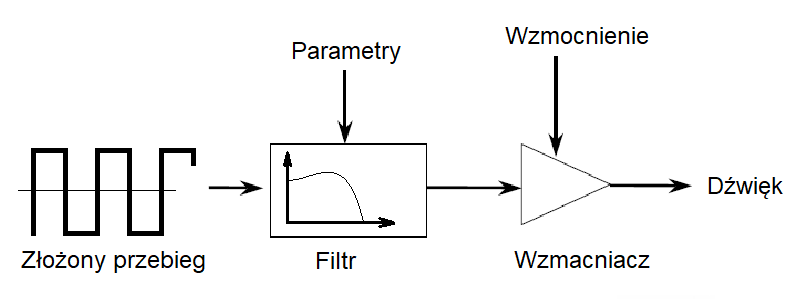
\includegraphics[width=12cm]{grafiki/sub_diagram}
	\captionsetup{justification=centering}
	\caption{Schemat blokowy dla metody subtraktywnej.}
	\label{rys:sub_diagram}
\end{figure}

Przykładowy wynik takiego działania przedstawiony jest na rysunku \ref{rys:sub_wykres1}.
\begin{figure}[H]
	\centering
	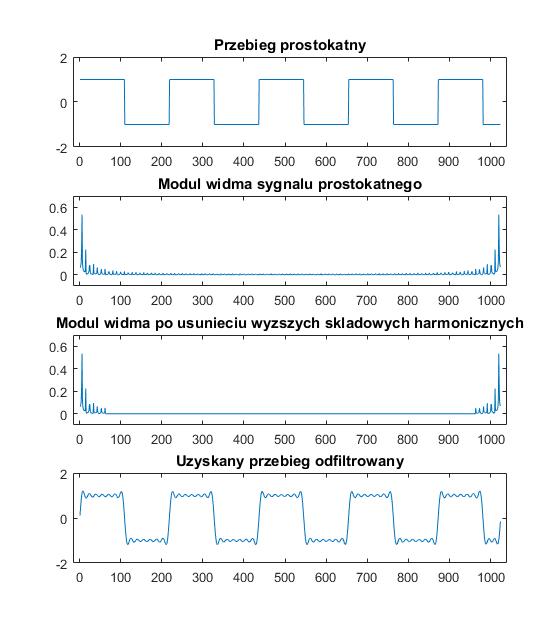
\includegraphics[width=12cm]{grafiki/sub_wykres1}
	\captionsetup{justification=centering}
	\caption{Zasada działania metody subtraktywnej.}
	\label{rys:sub_wykres1}
\end{figure}
Jak widać na \ref{rys:sub_wykres1}, na początku generowane jest 1024 próbek przebiegu prostokątnego. Następnie obliczane jest widmo tego sygnału. Z widma usuwane są wyższe składowe harmoniczne. Osiągnąć to można za pomocą filtracji idealnym filtrem dolnoprzepustowym. Przykład idealnego filtra dolnoprzepustowego opisanego w dziedzinie częstotliwości jako
\begin{equation} \label{equ:sub_lowpass}
H(\omega)=\left \{\begin{array}{ r l }
1, & \quad \text{$dla$ } \omega \leqslant \omega_{gr}\\
0, & \quad  \text{$dla$ } \omega > \omega_{gr}
\end{array}
\right.
\end{equation}
\begin{tabular}{ l l l l}
	gdzie: & $\omega$ &  - & pulsacja, \\
	&	$\omega_{gr}$ & - &  pulsacja graniczna filtru,\\
\end{tabular} \\ \\
przedstawiono na rysunku \ref{rys:sub_lowpass}. Pulsacja graniczna filtru to taka pulsacja, powyżej której wzmocnienie jest mniejsze niż 3 dB w stosunku do pasma przepustowego tego filtru. W przypadku idealnym wzmocnienie zmienia się skokowo z 1 na 0 dokładnie na pulsacji granicznej. W pokazanym przykładzie pulsacja graniczna wynosi około 6283 rad/s, co zgodnie ze wzorem
\begin{equation} \label{equ:sub_frequency}
f = \frac{\omega}{2 \pi}
\end{equation}
daje częstotliwość równą 1000 Hz.
\begin{figure}[H]
	\centering
	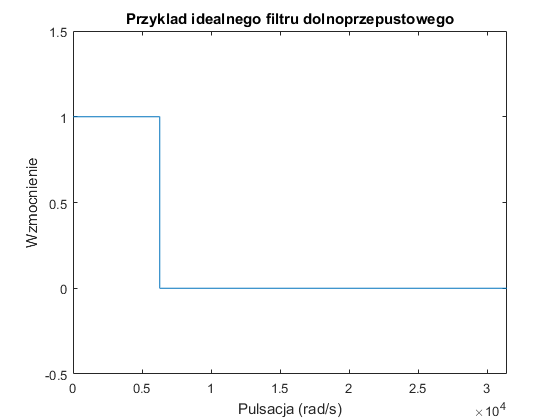
\includegraphics[width=8cm]{grafiki/sub_lowpass}
	\captionsetup{justification=centering}
	\caption{Idealny filtr dolnoprzepustowy.}
	\label{rys:sub_lowpass}
\end{figure}

Aby zadany sygnał przefiltrować pożądanym filtrem, należy wykonać operację splotu:
\begin{equation} \label{equ:sub_splot}
y(t)= h(t)*x(t) = \int_{0}^{t} h(\tau)x(t-\tau)d\tau
\end{equation}
\begin{tabular}{ l l l l}
	gdzie: & $y(t)$ &  - & wynik splotu, \\
	&	$h(t)$ & - &  odpowiedź impulsowa filtru,\\
	&	$x(t)$ & - &  filtrowany sygnał,\\
	
\end{tabular} \\ \\
który w przypadku dyskretnym jest zdefiniowany jako:
\begin{equation} \label{equ:sub_splot_dyskretny}
y[n]= h[n]*x[n] = \sum_{k=-\infty}^{\infty} h[k]x[n-k]
\end{equation}

Jedną z własności przekształcenia Fouriera jest to, że operacji splotu w dziedzinie czasu odpowiada operacja mnożenia w dziedzinie częstotliwości
\begin{equation} \label{equ:sub_splot_twierdzenie}
\mathcal{F}\{y(t)\} = \mathcal{F}\{h(t)*x(t)\} = H(\omega) X(\omega)
\end{equation}
\begin{tabular}{ l l l l}
	gdzie: & $\mathcal{F}\{y(t)\}$ &  - & transformata Fouriera wyniku splotu, \\
	&	$ H(\omega)$ & - &  transformata Fouriera odpowiedzi impulsowej filtru,\\
	&	$X(\omega)$ & - &  transformata Fouriera filtrowanego sygnału.\\
	
\end{tabular} \\ \\
Analogicznie, dla przypadku dyskretnego:
\begin{equation} \label{equ:sub_splot_twierdzenie_dyskretne}
\mathcal{F}\{y[n]\} = \mathcal{F}\{h[n]*x[n]\} = H(k) X(k).
\end{equation}
Oznacza to, że równoważnym do działania opisanego w \ref{equ:sub_splot_dyskretny} jest:
\begin{equation} \label{equ:sub_splot_dyskretny2}
y[n] = \mathcal{F}^{-1}\{ H(k) X(k)\} 
\end{equation}
Zatem z przefiltrowanego widma, za pomocą odwrotnej transformacji Fouriera, obliczany jest przebieg czasowy. W pokazanym przykładzie na \ref{rys:sub_wykres1}, w wyniku otrzymuje się sygnał prostokątny po filtracji dolnoprzepustowej.
\section{Implementacja syntezy subtraktywnej}
W przypadku syntezatorów analogowych, poszczególne bloki są realizowane za pomocą elementów elektronicznych takich jak oscylatory (VCO) oraz przestrajalne filtry. W syntezatorach cyfrowych implementacje mogą być różne, jednak muszą być na tyle wydajne obliczeniowo, aby dana platforma sprzętowa poradziła sobie z syntezą dźwięku w czasie rzeczywistym bez artefaktów dźwiękowych. W tym podrozdziale opisana zostanie obrana droga implementacji metody subtraktywnej na procesorze sygnałowym. 
Próbki sygnału są syntezowane w sposób blokowy. Blok danych składa się z $N=1024$ próbek.

\subsection{Generowanie przebiegu}
W dwóch tablicach o $N$ elementach przechowywane są kolejne próbki sygnału podstawowego, czyli sygnału bogatego w wyższe składowe harmoniczne. Po dokonaniu filtracji i wystawieniu próbek jednej z tablic na przetwornik cyfrowo-analogowy, wystawiane są próbki z drugiej tablicy. W tym czasie w chwilowo nieużywanej tablicy należy wygenerować kolejne 1024 próbek sygnału. Trzeba przy tym pamiętać o odpowiednim przesunięciu fazowym, tak aby zachować ciągłość pomiędzy kolejnymi blokami próbek wystawianych na przetwornik. Równanie \ref{equ:sub_1} opisuje sposób generowania przebiegu prostokątnego.
\begin{equation} \label{equ:sub_1}
waveform[i]=\left \{\begin{array}{ r l }
1, & \quad \text{$dla$ } sin(2\pi f\frac{k+i}{F_s}) > 0\\
-1, & \quad  \text{$dla$ } sin(2\pi f\frac{k+i}{F_s}) \leqslant 0
\end{array}
\right.
\end{equation}
\begin{tabular}{ l l l l}
	gdzie: & $waveform$ &  - & tablica zmiennych typu float, \\
	&	$f$ & - &  pożądana częstotliwość generowanego przebiegu, \\
	&	$F_s$ & - & częstotliwość próbkowania,\\
	&	$i$ & - &  licznik iteracji, $i$ = 1, 2, 3, ..., N,\\
	&	$k$ & - &  licznik bloków.\\
\end{tabular} \\ \\
Po wyznaczeniu każdego bloku próbek, zwiększany jest licznik bloków $k$:
\begin{equation} \label{equ:sub_2}
k = k_{old} + N.
\end{equation}
Na rysunku \ref{rys:sub_waveform_blocks} pokazano dwa kolejne bloki próbek wygenerowanego przebiegu prostokątnego. Dzięki odpowiedniemu przesunięciu fazowemu przebiegi te, po wystawieniu na przetwornik cyfrowo-analogowy, utworzą ciągły dźwięk - bez trzasków.
\begin{figure}[H]
	\centering
	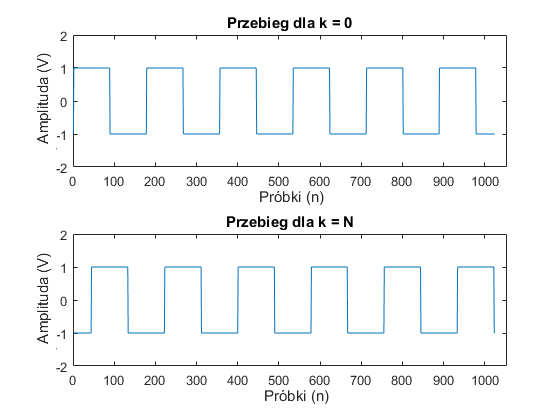
\includegraphics[width=12cm]{grafiki/sub_waveform_blocks}
	\captionsetup{justification=centering}
	\caption{Dwa kolejne bloki próbek przebiegu prostokątnego.}
	\label{rys:sub_waveform_blocks}
\end{figure}

\subsection{DFT i filtracja sygnału}
Na podstawie wygenerowanych próbek przebiegu oblicza się DFT za pomocą algorytmu FFT. W wyniku otrzymuje się $N$ liczb zespolonych. Przechowywane są one w tablicy o rozmiarze $2N$ w taki sposób, że każdy element o indeksie parzystym to część rzeczywista próbki, a sąsiadujący z nią element o indeksie nieparzystym to część urojona tej próbki. Filtracja dokonywana jest poprzez wyzerowanie elementów o odpowiednich indeksach. Na przykład filtracja dolnoprzepustowa z częstotliwością graniczną o wartości 1400 Hz dokonywana jest według poniżego wzoru:
\begin{equation} \label{equ:sub_3}
waveform_{fft}[i]=\left \{\begin{array}{ r l }
0, & \quad  \text{dla } N - f_g \leqslant \frac{i}{2} \leqslant N + f_g \\
waveform_{fft}[i], & \quad \text{w pozostałych przypadkach } 

\end{array}
\right.
\end{equation}
\begin{tabular}{ l l l l}
	gdzie: & $waveform_{fft}$ &  - & próbki transformaty Fouriera sygnału, \\
	&	$freq$ & - &  częstotliwość przeliczona na indeksy w tablicy, $freq = N - 2 \frac{1400N}{Fs} - 1$, \\
	&	$F_s$ & - & częstotliwość próbkowania,\\
	&	$i$ & - &  indeks, $i$ = 1, 2, 3, ..., 2N.\\
\end{tabular} \\ \\

Efekt tego typu filtracji można zobaczyć na drugim i trzecim wykresie na \ref{rys:sub_wykres1}. W analogiczny sposób dokonuje się pozostałych filtracji: górnoprzepustowej, pasmo-przepustowej i pasmo-zaporowej.

\subsection{Zakładkowanie bloków danych}
Samo przesuwanie w fazie generowanych sygnałów opisanych w \ref{equ:sub_2} nie rozwiązuje wszystkich problemów. Jak widać na ostatnim wykresie na \ref{rys:sub_wykres1}, uzyskany sygnał na końcu ma niespodziewany przebieg. Po połączeniu tego bloku próbek z następnym blokiem otrzyma się sygnał pokazany na rysunku \ref{rys:sub_zakladkowania_brak}.
\begin{figure}[H]
	\centering
	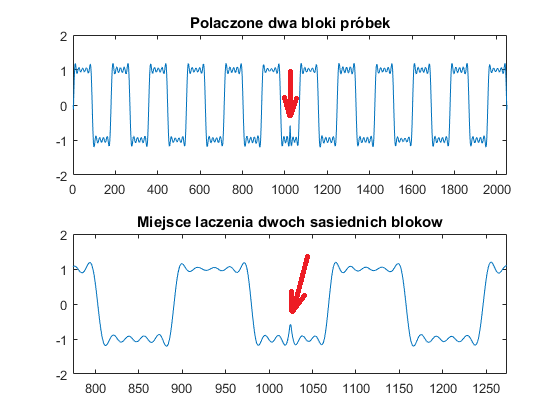
\includegraphics[width=12cm]{grafiki/sub_zakladkowania_brak}
	\captionsetup{justification=centering}
	\caption{Dwa kolejne bloki próbek przebiegu prostokątnego.}
	\label{rys:sub_zakladkowania_brak}
\end{figure}
Rozwiązaniem tego problemu jest zakładkowanie każdych dwóch sąsiednich bloków próbek. Zakładkowanie polega na nasunięciu pewnej liczby $m$ początkowych próbek następnego bloku, na $m$ końcowych próbek bieżącego. W miejscach, gdzie bloki są na siebie nałożone, wartość każdej próbki obliczana jest jako średnia ważona z dwóch nałożonych na siebie próbek. Przy czym suma wag w każdej chwili czasu jest równa 1, wagi próbek bloku bieżącego maleją wraz z czasem, natomiast wagi próbek bloku następnego narastają. Najprostszym rozwiązaniem (a zatem efektywnym obliczeniowo) są wagi liniowe. Oznacza to, że wagi dla $m$ ostatnich lub pierwszych próbek bloku odpowiednio: liniowo maleją od 1 do 0 lub liniowo rosną od 0 do 1.
Nakładane na siebie próbki muszą odpowiadać sygnałowi w tej samej fazie, zatem należy zmodyfikować przesunięcie fazowe opisane przez \ref{equ:sub_2} do postaci:
\begin{equation} \label{equ:sub_4}
k = k_{old} + N - m.
\end{equation}
Porównanie zakładkowania dla różnych wartości $m$ przedstawiono na rysunku  \ref{rys:sub_overlaps}.
\begin{figure}[H]
	\centering
	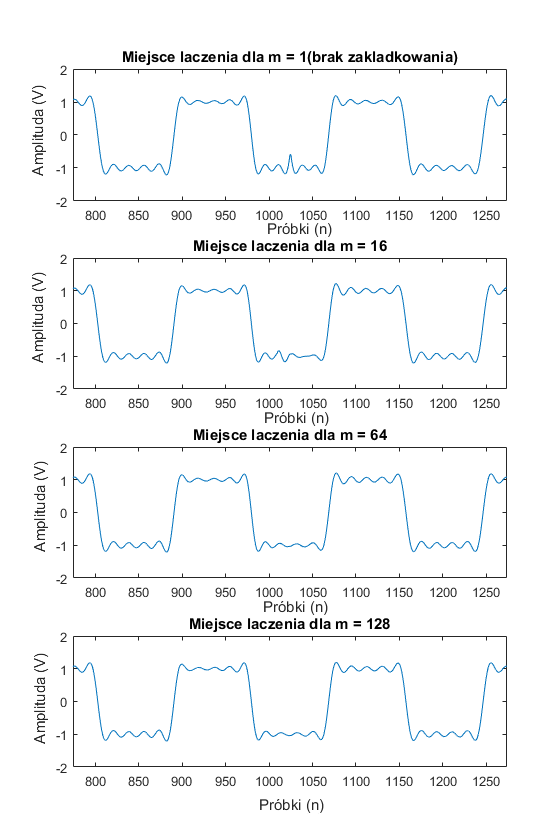
\includegraphics[width=10cm]{grafiki/sub_overlaps}
	\captionsetup{justification=centering}
	\caption{Wyniki zakladkowania przy zmiennej dlugosci zakladek.}
	\label{rys:sub_overlaps}
\end{figure}

Takie podejście wymusza użycie dwóch tablic ze zmiennymi typu float, w których przechowywane są próbki sygnału do wystawienia na przetwornik cyfrowo-analogowy. Wynika to z faktu, że w pewnych chwilach na DAC należy wystawić ważoną średnią próbek z dwóch różnych sygnałów. 

\subsection{Polifonia w syntezie subtraktywnej}
Powyższe rozważania dotyczyły syntezy pojedynczych tonów. Polifonię w danym podejściu, można osiągnąć korzystając z faktu, że przekształcenie Fouriera jest przekształceniem liniowym \cite{schafer}. Oznacza to, że jeśli
 \begin{equation} \label{equ:sub_5}
 \mathcal{F}\{x_n\} = X_k
 \end{equation}
 oraz 
  \begin{equation} \label{equ:sub_6}
 \mathcal{F}\{y_n\} = Y_k
 \end{equation}
 wówczas
  \begin{equation} \label{equ:sub_7}
\mathcal{F}\{ax_n + by_n\} = aX_k + bY_k.
\end{equation} 
Zatem w programie na DSP, zamiast obliczać ciągle DFT, filtrację oraz IDFT tyle razy, ile użytkownik naciska klawiszy, można utworzyć sygnał będący sumą przebiegów podstawowych. Dopiero taki sygnał poddawany będzie dalszemu przetwarzaniu. Na rysunku \ref{rys:sub_linearity}	zobrazowana została własność liniowości przekształcenia Fouriera. Na pierwszych trzech wykresach pokazane zostały 3 przebiegi prostokątne o różnych częstotliwościach. W drugim rzędzie widnieją te przebiegi po przepuszczeniu przez filtr dolnoprzepustowy. W trzecim rzędzie znajduje się przebieg, który jest sumą początkowych przebiegów prostokątnych (przed filtracją). W ostatnim rzędzie pokazano sumę tych przefiltrowanych przebiegów oraz przebieg z rzędu trzeciego po filtracji dolnoprzepustowej takim samym filtrem. Przykład ten pokazuje, że obie drogi prowadzą do tych samych wyników.
\begin{figure}[H]
	\centering
	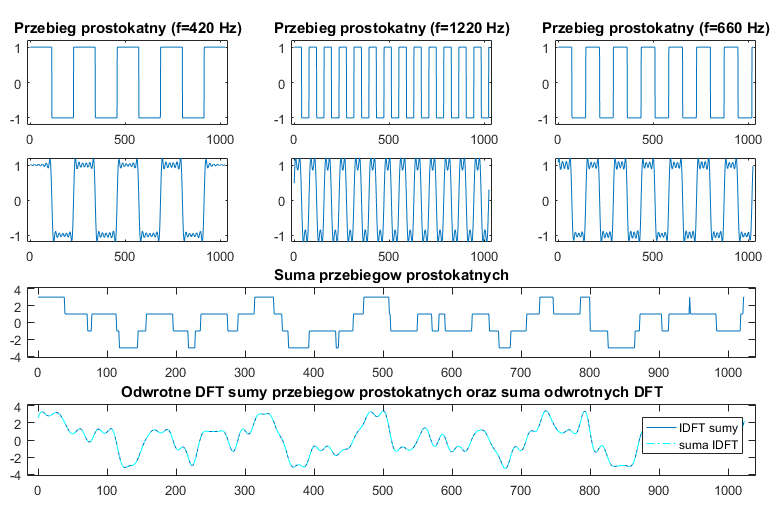
\includegraphics[width=16cm]{grafiki/sub_linearity}
	\captionsetup{justification=centering}
	\caption{Własność liniowości przekształcenia Fouriera.}
	\label{rys:sub_linearity}
\end{figure}

\section{Interfejs użytkownika}
Przy syntezie subtraktywnej, użytkownik powinien mieć możliwość samodzielnego wyboru przebiegów podstawowych generowanych przy naciskaniu klawiszy oraz strojenia filtrów, które ten przebieg filtrować będą. W przypadku filtrów idealnych, jedyne co musi określić użytkownik dla ich działania, to ich częstotliwości graniczne.
\begin{figure}[H]
	\centering
	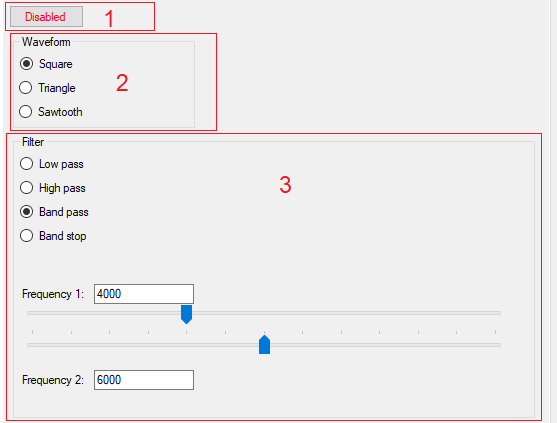
\includegraphics[width=12cm]{grafiki/sub_interface}
	\captionsetup{justification=centering}
	\caption{Interfejs użytkownika dla syntezy subtraktywnej.}
	\label{rys:sub_interface}
\end{figure}
Na rysunku \ref{rys:sub_interface} zaznaczono trzy sekcje wykonanego interfejsu dla syntezy subtraktywnej. W pierwszej z nich znajduje się przycisk, który służy do aktywacji tej metody syntezy dźwięku. Po naciśnięciu tego klawisza, DSP otrzymuje komunikat, po którym przechodzi w tryb syntezy subtraktywnej.

W sekcji drugiej znajdują się rodzaje przebiegów podstawowych, spośród których użytkownik może wybrać tylko jeden w danej chwili. Zaznaczenie dowolnego z nich zmienia w programie DSP odpowiednią flagę. Gdy następnie zostanie naciśnięty klawisz, wygenerowany zostanie właśnie taki przebieg podstawowy, jaki jest w interfejsie zaznaczony.

W trzeciej sekcji znajdują rodzaje filtrów oraz suwaki pozwalające na wybór częstotliwości granicznych: dolnej, górnej lub obu jednocześnie - zależnie od wybranego rodzaju filtra. Podobnie jak przy wyborze rodzaju przebiegu podstawowego - tutaj również użytkownik zaznacza jeden z rodzajów filtra. W zależności od wybranego filtra, odblokowane zostaną odpowiednie suwaki pozwalające mieniać częstotliwości graniczne. Na przykład, dla filtra dolnoprzepustowego odblokowany zostanie tylko suwak dolny, gdyż to on odpowiada za częstotliwość graniczną górną. Natomiast dla filtru pasmo-przepustowego odblokowane zostaną oba suwaki, a pasmo przepustowe zawierać się będzie pomiędzy wskazaniem suwaka górnego - częstotliwości granicznej dolnej oraz suwaka dolnego - częstotliwości granicznej górnej.
Zmian częstotliwości można dokonywać na dwa sposoby:
\begin{itemize}
	\item za pomocą suwaków. W tym wypadku wartość ustawiona za pomocą suwaka zostanie automatycznie wpisana do pola tekstowego skojarzonego z tym suwakiem.
	\item Poprzez precyzyjne wpisanie wartości do pola tekstowego obok suwaka. W tej sytuacji suwak automatycznie się przesunie na pozycję odpowiadającą wpisanej wartości.
\end{itemize}
\section{Wyniki}

